\documentclass{paper}


\usepackage{epsfig}
\usepackage{graphicx}
\usepackage{amsmath}
\usepackage{amssymb}
\usepackage{amsthm}

\usepackage{color}
\usepackage{subcaption}
\usepackage{caption}




\usepackage{mathrsfs}
\usepackage{algpseudocode}
\usepackage{algorithm}

\usepackage{float}
\usepackage{mathtools}
\usepackage{mdwlist}
\usepackage{gensymb}
\usepackage{array}
\usepackage{multirow}
\usepackage[hmargin=3cm]{geometry}
\usepackage{boxedminipage}
\usepackage{enumerate}


\setlength{\parindent}{0pt}
\setlength{\parskip}{18pt}


\usepackage[latin1]{inputenc} 
\usepackage[T1]{fontenc} 

\usepackage{listings} 
\lstset{% 
   language=Matlab, 
   basicstyle=\small\ttfamily, 
} 






\renewcommand{\algorithmicforall}{\textbf{Foreach}}
\newcommand{\init}{\textbf{INIT }}
\newcommand{\pluseq}{\mathrel{+}=}
\newcommand{\asteq}{\mathrel{*}=}
\newcommand{\myto}{\textbf{TO }}
\newcommand*\colvec[3][]{
    \begin{pmatrix}\ifx\relax#1\relax\else#1\\\fi#2\\#3\end{pmatrix}
}
\newcommand{\myparagraph}[1]{\paragraph{#1}\mbox{}\\}
\DeclarePairedDelimiter\ceil{\lceil}{\rceil}
\DeclarePairedDelimiter\floor{\lfloor}{\rfloor}



\title{Computational Photography Assignment 5}



\author{Single Michael\\08-917-445}
% //////////////////////////////////////////////////


\begin{document}



\maketitle


\section{Morphing}
The following figures show some static results produced by my morphing function. I also have produced some .avi movies. You can find them either in \emph{outputs/p5/} or in the provided results zip on Ilias. I rendered the movies once using a linear time-stepping function and another time using a cosine-ramp. Furthermore, for my results, I used 42 frames. The duration of the movies is 3 seconds. In order to make your own morphing videos, please make use of the function \emph{makeMorphingVideo.m} and read its description (how to use).

\begin{figure}[H]
    \centering
    \begin{subfigure}{0.45\textwidth}
        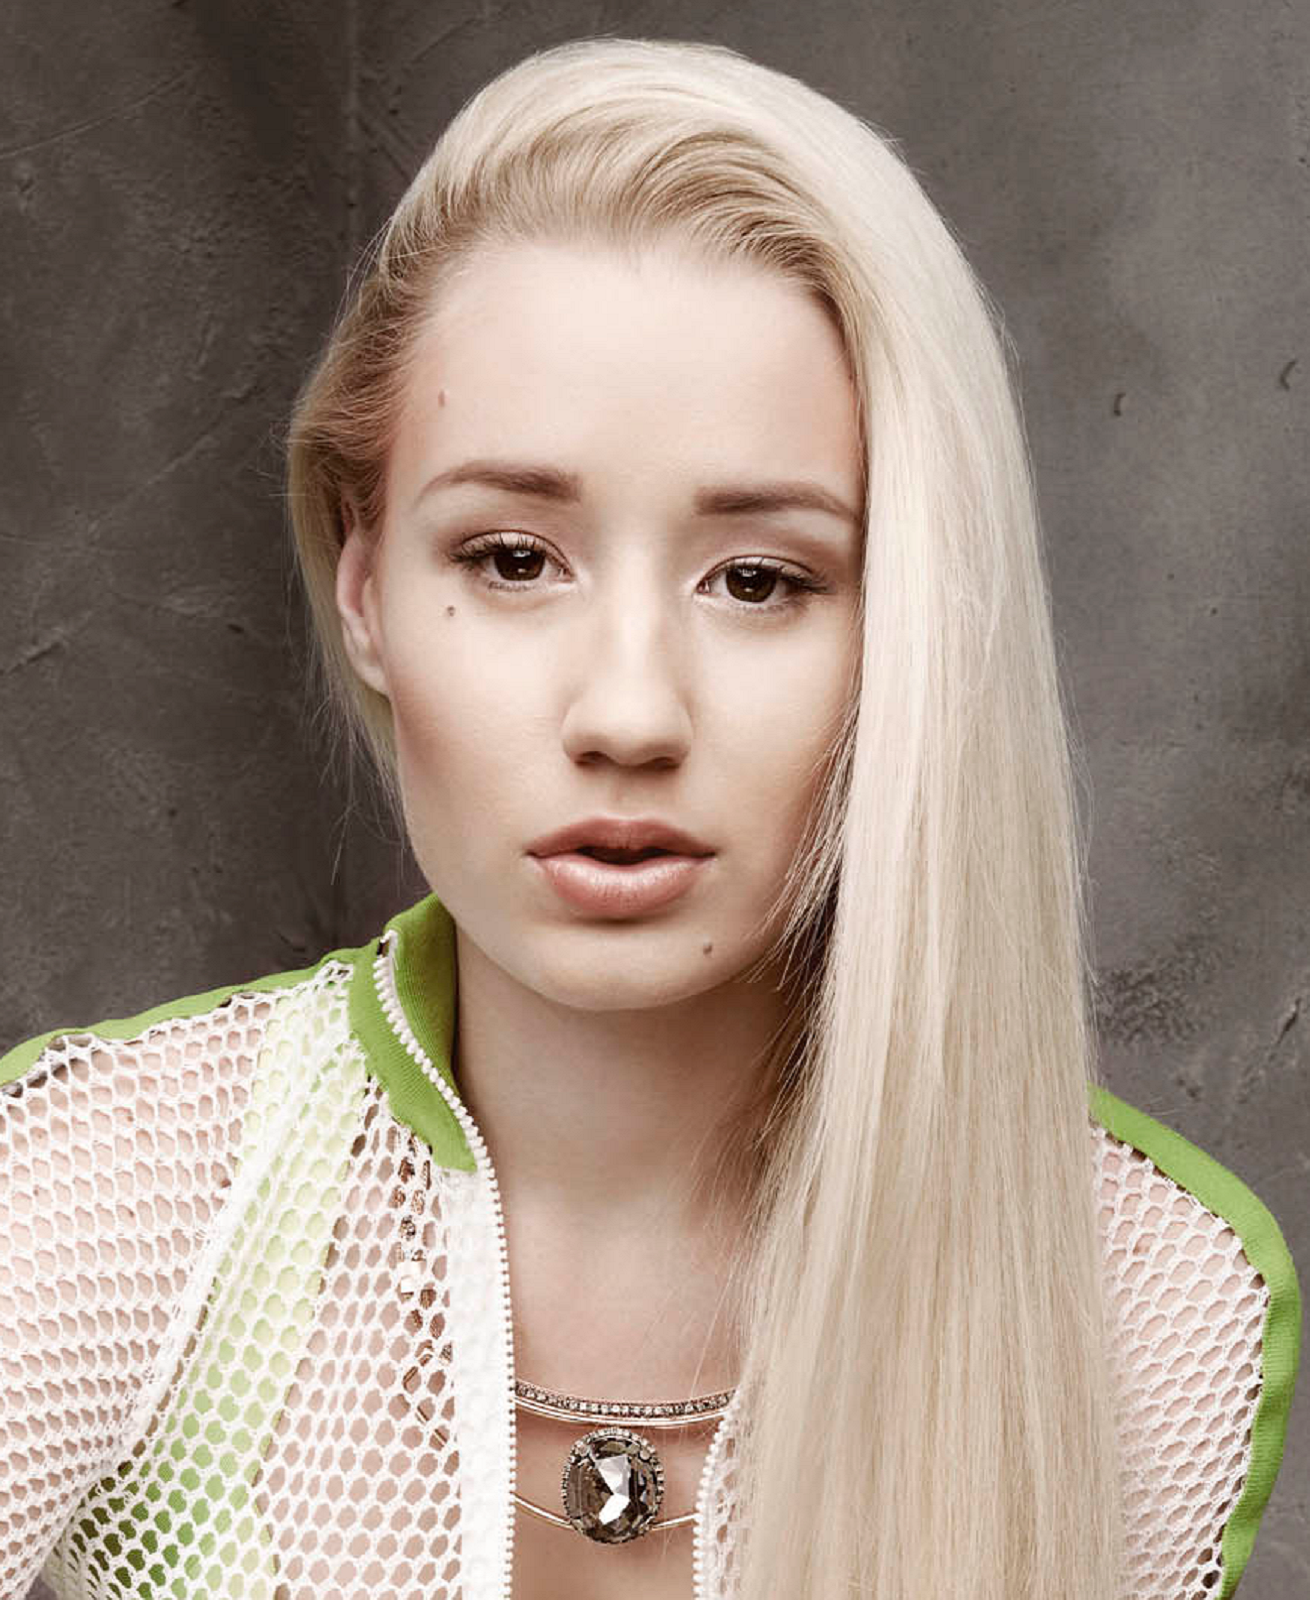
\includegraphics[width=\textwidth]{morph/from}
    \end{subfigure}
    ~
        \begin{subfigure}{0.45\textwidth}
        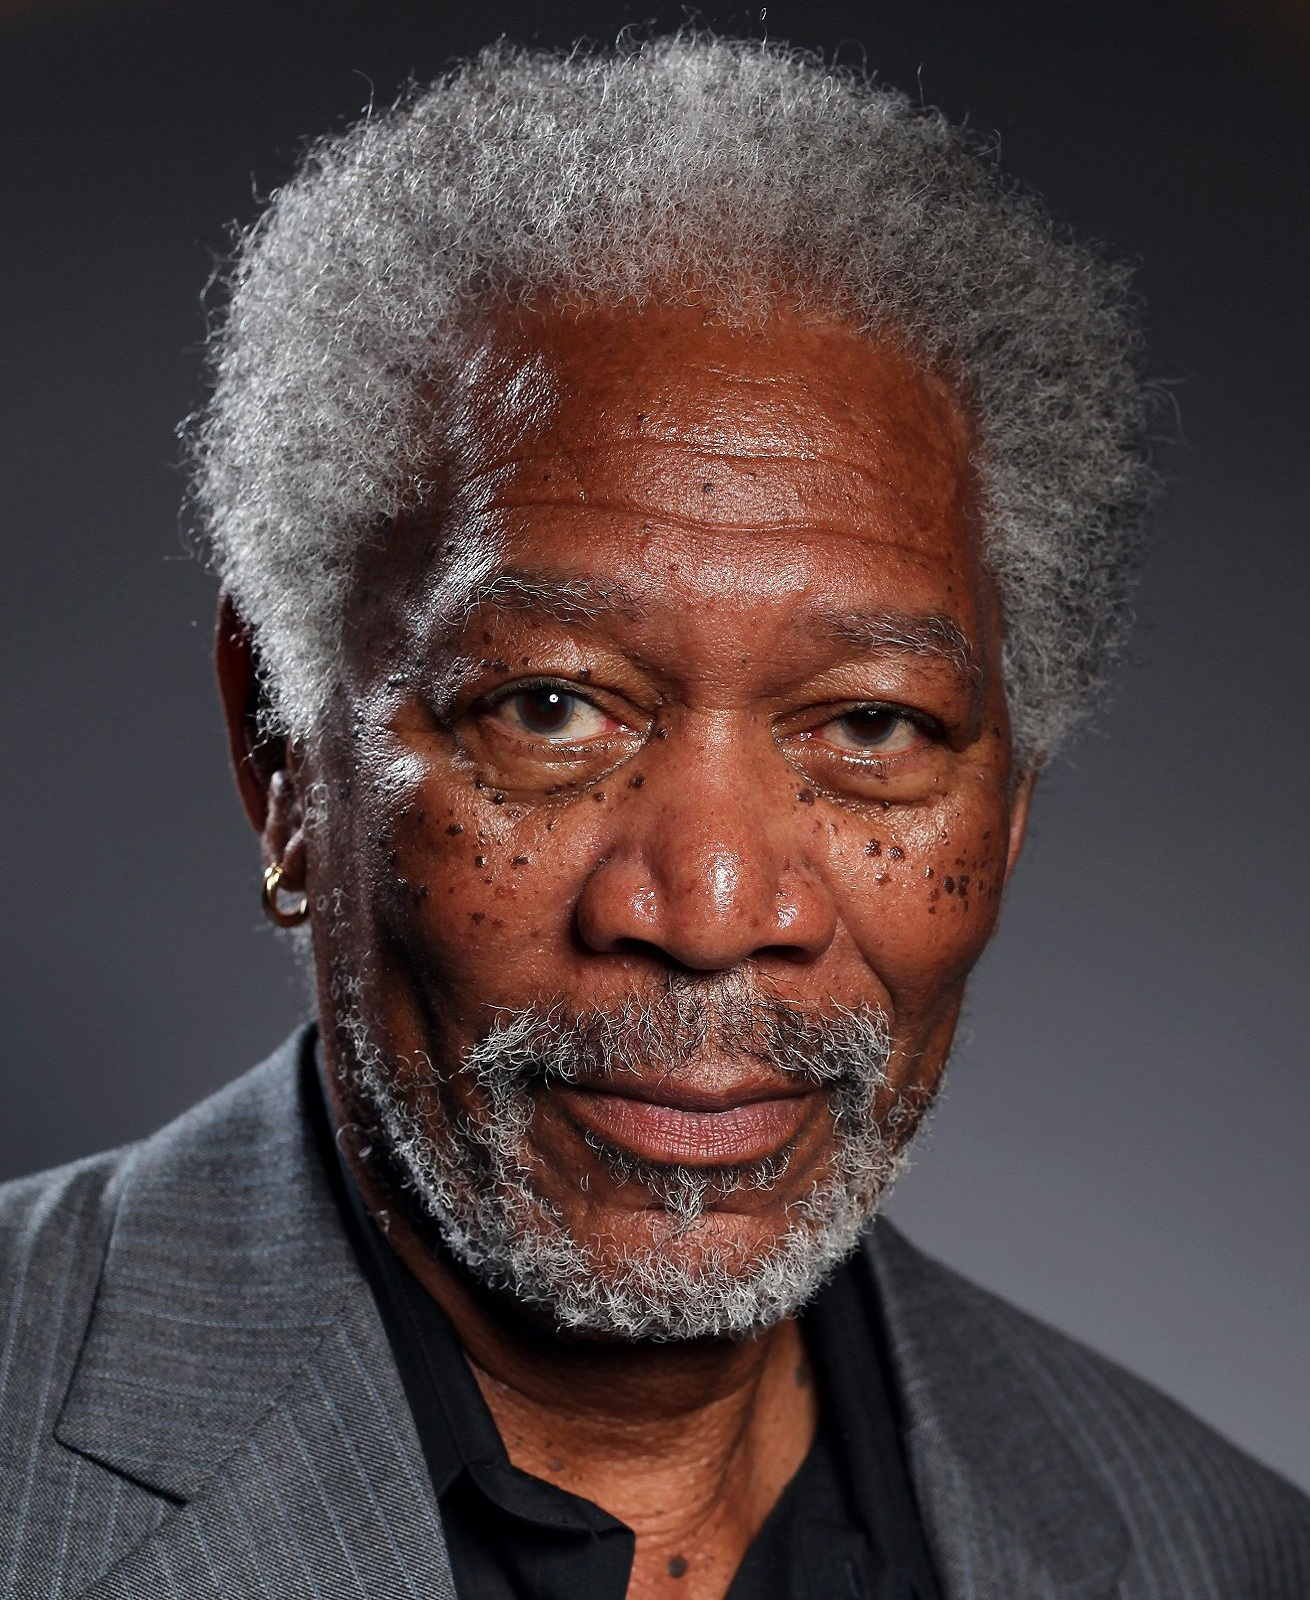
\includegraphics[width=\textwidth]{morph/to}
    \end{subfigure}
    
    \caption{Source Image (left) and target image (right) used for morphing.}
    \label{fig:morphing_input}       
\end{figure}

\begin{figure}[H]
    \centering
    \begin{subfigure}{0.45\textwidth}
        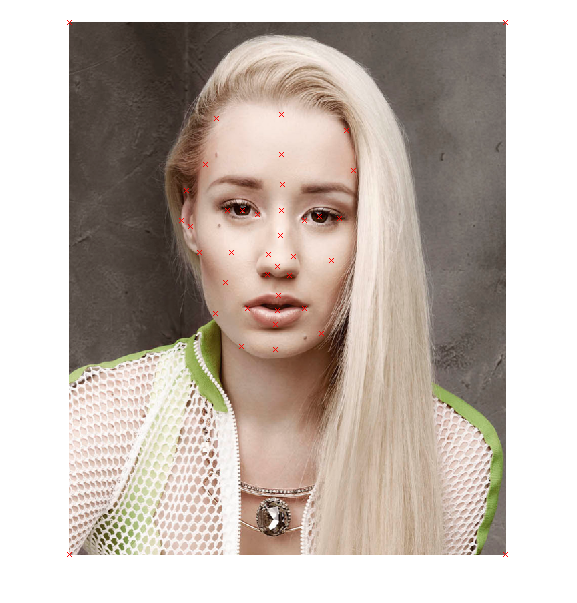
\includegraphics[width=\textwidth]{morph/selected_features_source}
    \end{subfigure}
    ~
        \begin{subfigure}{0.45\textwidth}
        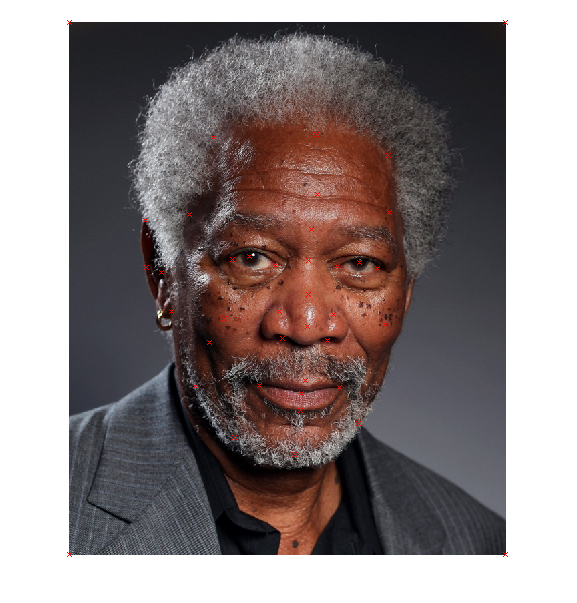
\includegraphics[width=\textwidth]{morph/selected_features_target}
    \end{subfigure}
    
    \caption{Selected Features in Source Image (left) and Selected Features in Target Image (right) used for morphing indicated by red crosses.}
    \label{fig:morphing_selected_features}       
\end{figure}

\begin{figure}[H]
    \centering
    \begin{subfigure}{0.45\textwidth}
        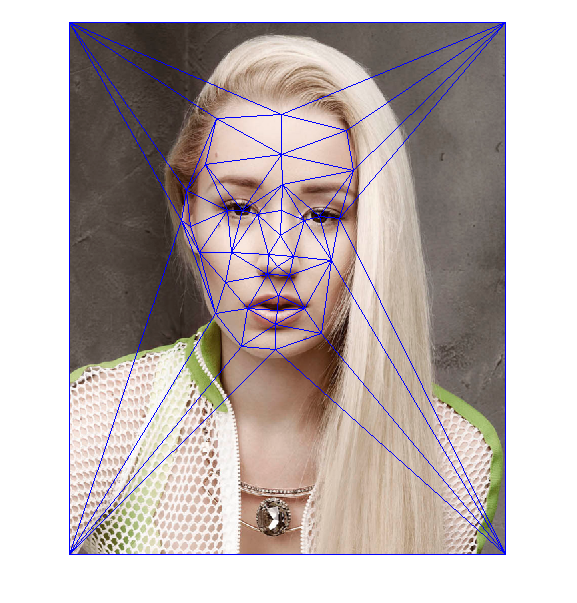
\includegraphics[width=\textwidth]{morph/triangulation_source}
    \end{subfigure}
    ~
        \begin{subfigure}{0.45\textwidth}
        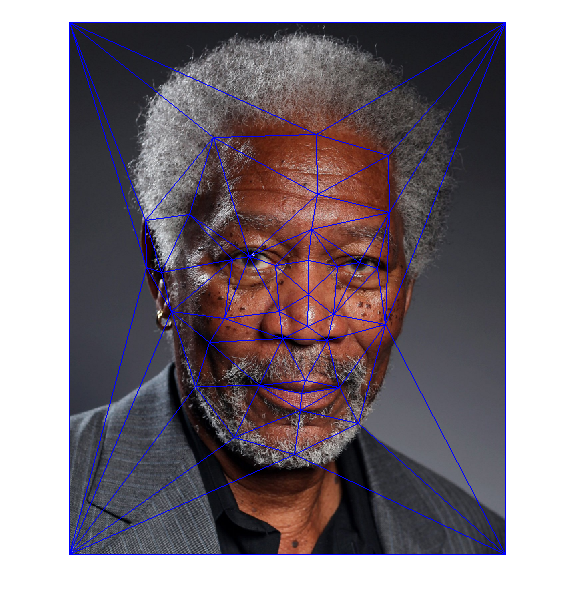
\includegraphics[width=\textwidth]{morph/triangulation_target}
    \end{subfigure}
    
    \caption{Delaunay triangulation using selected features in Source image (left) and Delaunay triangulation using selected features in Target image  (right) used for morphing.}
    \label{fig:morphing_delaunay}       
\end{figure}

\begin{figure}[H]
    \centering
    \begin{subfigure}{1.0\textwidth}
        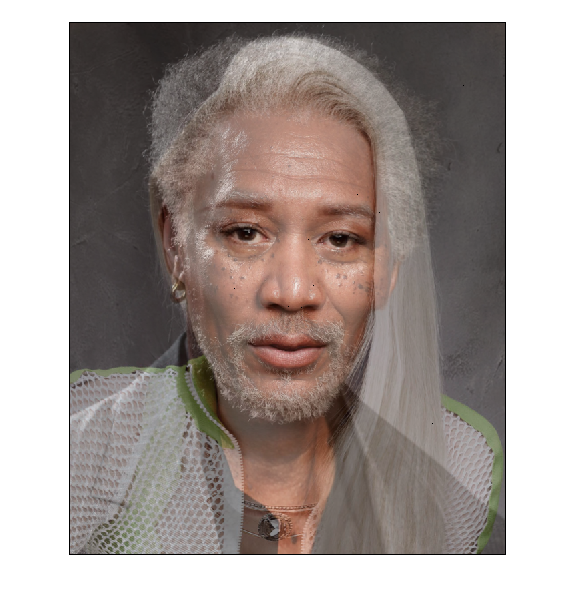
\includegraphics[width=\textwidth]{morph/intermediate_morph}
    \end{subfigure}
    
    \caption{An intermediate morphed image (between source and target) using linear timesteps. here t is equal 0.5.}
    \label{fig:morphing_intermediate}       
\end{figure}

\section{Rectification using Homography}
Figure $\ref{fig:rectify_input_building}$ is the example shown during the exercise session. Its result, when applying a rectification is shown in figure $\ref{fig:rectified_building}$. This example acts as a sanity check whether my implementation seems to work as expected. In addition I have produced rendering for another example, a distorted church shown in figure $    \ref{fig:rectify_input_skewed_church}$. Figure $\ref{fig:rectify_selection_skewed_church}$illustrated the user selection for the rectification process (used for computing the homography). Figure $ \ref{fig:rectified_skewed_church}$shows the result of the homographic image rectification applied to this church image. \\

In order to make your own rectification, please make use of the function \emph{homographicRectification.m} and read its description (how to use).


\begin{figure}[H]
    \centering
    \begin{subfigure}{1.0\textwidth}
        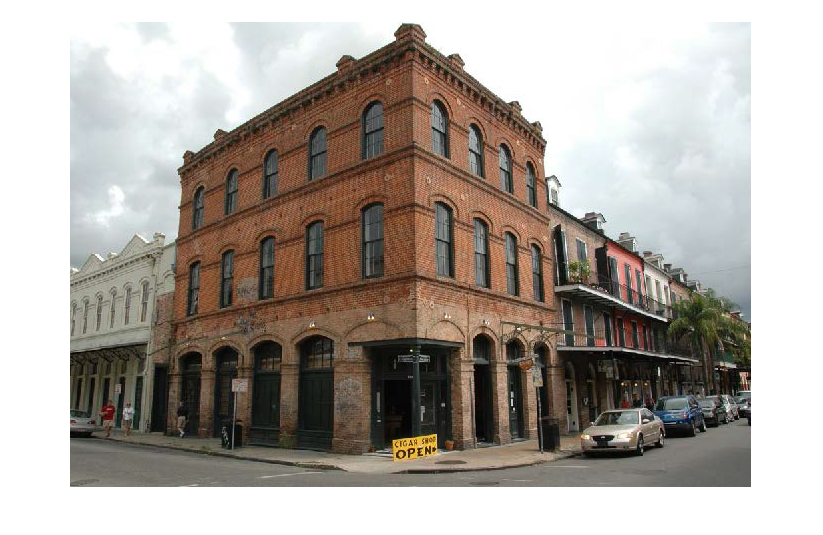
\includegraphics[width=\textwidth]{rectify/input_building}
    \end{subfigure}
    
    \caption{Input image of a building which exhibits a notable distortion.}
    \label{fig:rectify_input_building}       
\end{figure}

\begin{figure}[H]
    \centering
    \begin{subfigure}{1.0\textwidth}
        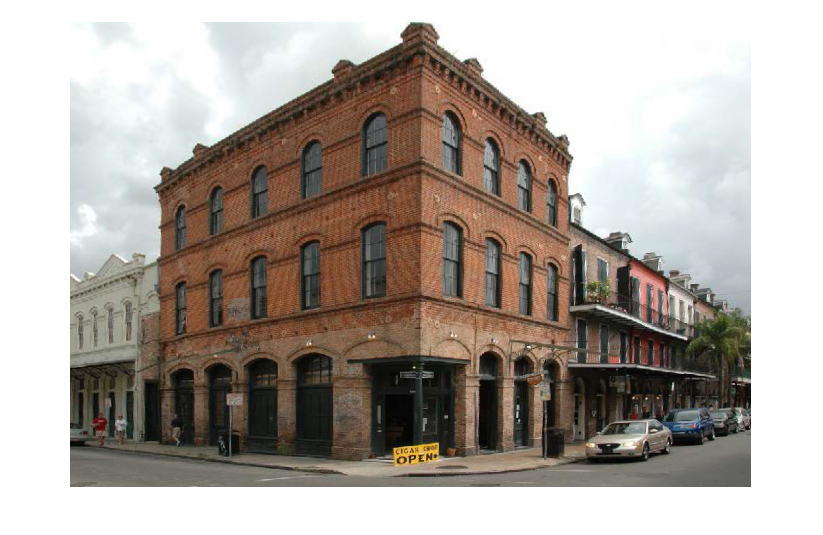
\includegraphics[width=\textwidth]{rectify/rectified_building}
    \end{subfigure}
    
    \caption{Rectified input image using Homography. Most of the vertical edges of the building have become parallel. }
    \label{fig:rectified_building}       
\end{figure}


\begin{figure}[H]
    \centering
    \begin{subfigure}{1.0\textwidth}
        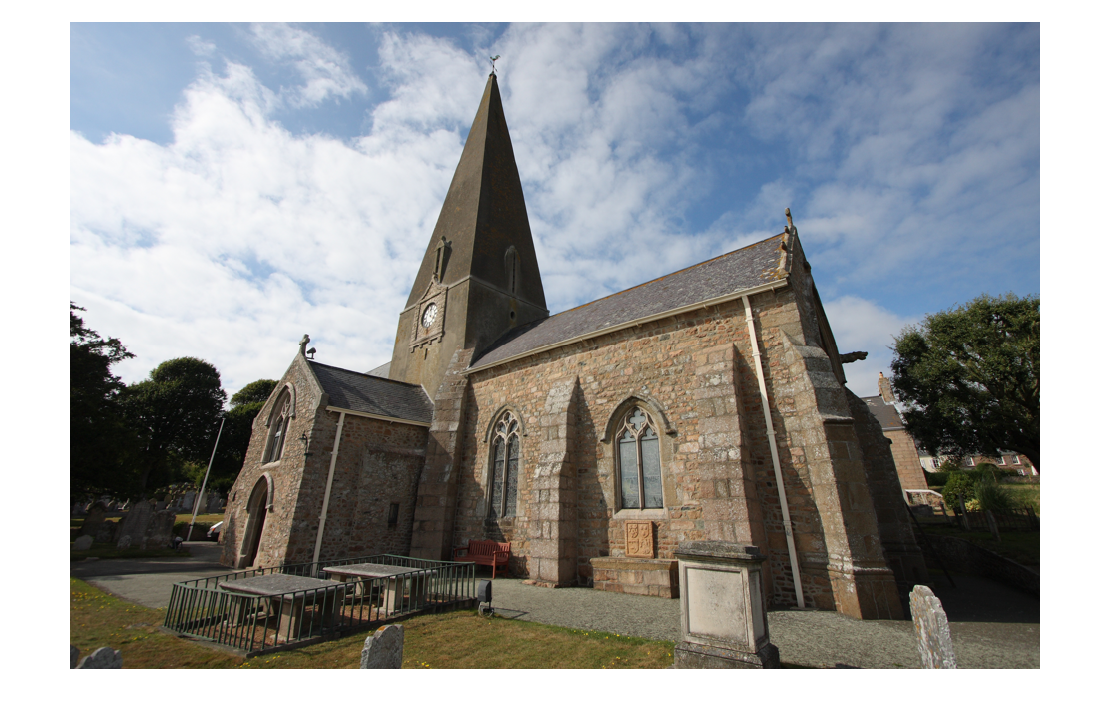
\includegraphics[width=\textwidth]{rectify/input_skewed_church}
    \end{subfigure}
    
    \caption{Input image of a church which exhibits a notable distortion.}
    \label{fig:rectify_input_skewed_church}       
\end{figure}

\begin{figure}[H]
    \centering
    \begin{subfigure}{1.0\textwidth}
        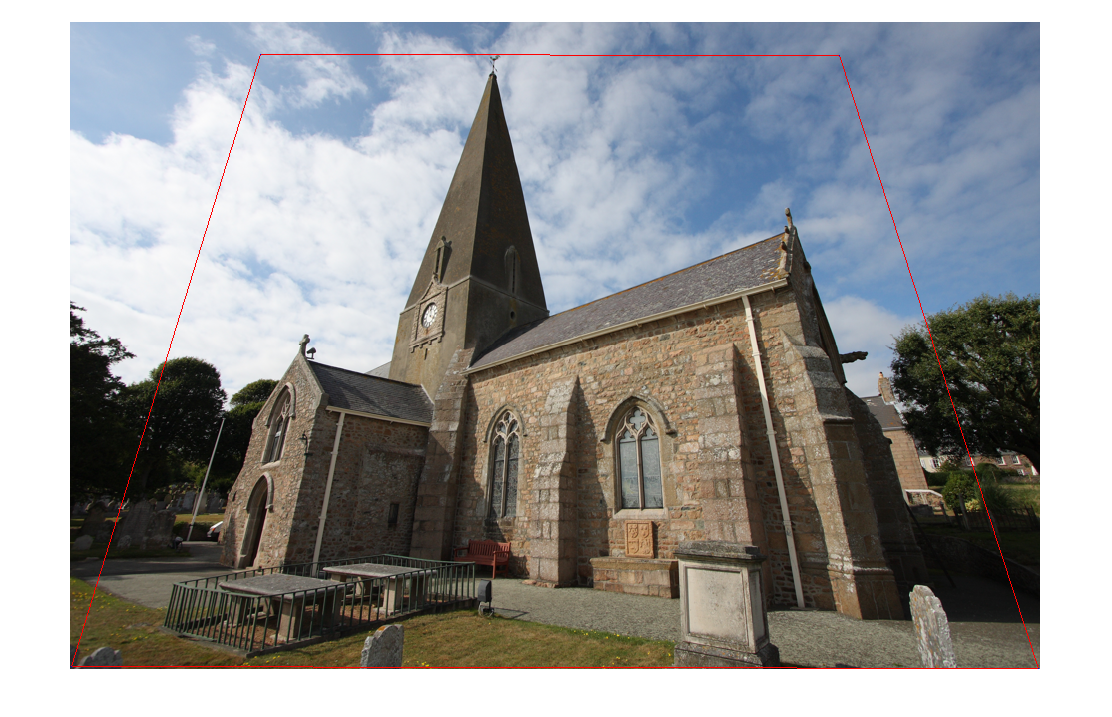
\includegraphics[width=\textwidth]{rectify/selection_skewed_church}
    \end{subfigure}
    
    \caption{Image Rectification selection (read lines) from specified user points (in blue).}
    \label{fig:rectify_selection_skewed_church}       
\end{figure}

\begin{figure}[H]
    \centering
    \begin{subfigure}{1.0\textwidth}
        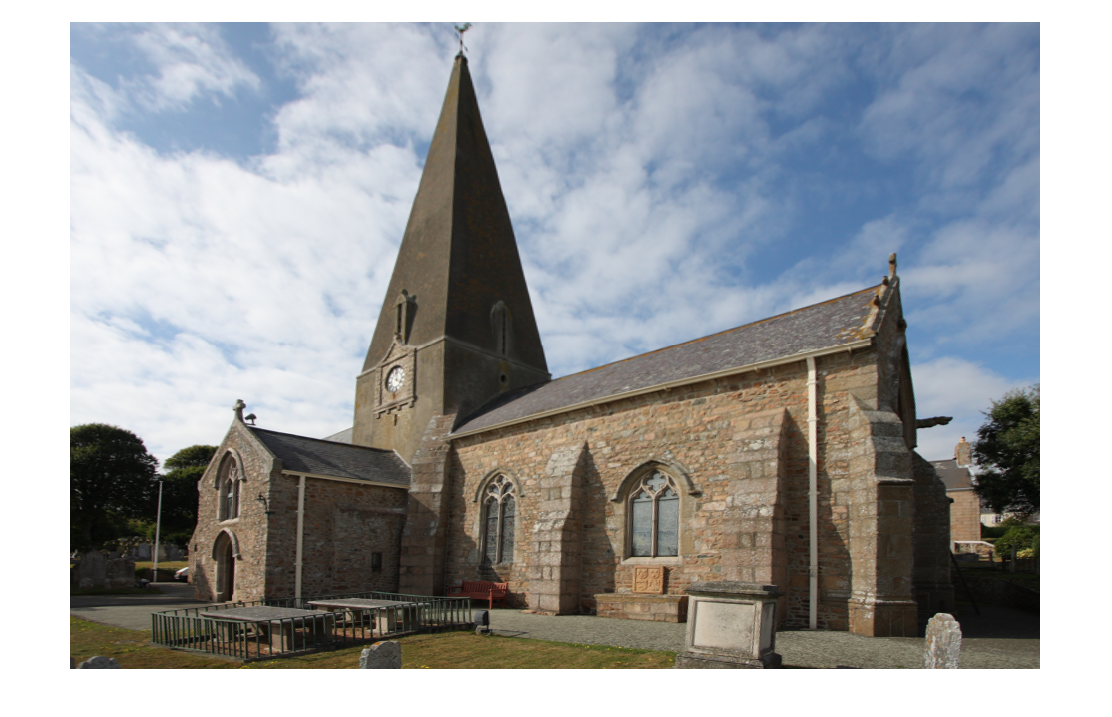
\includegraphics[width=\textwidth]{rectify/rectified_skewed_church}
    \end{subfigure}
    
    \caption{Rectified input image using Homography. Most of the vertical edges of the church have become parallel. }
    \label{fig:rectified_skewed_church}       
\end{figure}








\section{Panorama Stitching}




\end{document}